% Options for packages loaded elsewhere
\PassOptionsToPackage{unicode}{hyperref}
\PassOptionsToPackage{hyphens}{url}
%
\documentclass[
]{article}
\usepackage{amsmath,amssymb}
\usepackage{iftex}
\ifPDFTeX
  \usepackage[T1]{fontenc}
  \usepackage[utf8]{inputenc}
  \usepackage{textcomp} % provide euro and other symbols
\else % if luatex or xetex
  \usepackage{unicode-math} % this also loads fontspec
  \defaultfontfeatures{Scale=MatchLowercase}
  \defaultfontfeatures[\rmfamily]{Ligatures=TeX,Scale=1}
\fi
\usepackage{lmodern}
\ifPDFTeX\else
  % xetex/luatex font selection
\fi
% Use upquote if available, for straight quotes in verbatim environments
\IfFileExists{upquote.sty}{\usepackage{upquote}}{}
\IfFileExists{microtype.sty}{% use microtype if available
  \usepackage[]{microtype}
  \UseMicrotypeSet[protrusion]{basicmath} % disable protrusion for tt fonts
}{}
\makeatletter
\@ifundefined{KOMAClassName}{% if non-KOMA class
  \IfFileExists{parskip.sty}{%
    \usepackage{parskip}
  }{% else
    \setlength{\parindent}{0pt}
    \setlength{\parskip}{6pt plus 2pt minus 1pt}}
}{% if KOMA class
  \KOMAoptions{parskip=half}}
\makeatother
\usepackage{xcolor}
\usepackage[margin=1in]{geometry}
\usepackage{graphicx}
\makeatletter
\def\maxwidth{\ifdim\Gin@nat@width>\linewidth\linewidth\else\Gin@nat@width\fi}
\def\maxheight{\ifdim\Gin@nat@height>\textheight\textheight\else\Gin@nat@height\fi}
\makeatother
% Scale images if necessary, so that they will not overflow the page
% margins by default, and it is still possible to overwrite the defaults
% using explicit options in \includegraphics[width, height, ...]{}
\setkeys{Gin}{width=\maxwidth,height=\maxheight,keepaspectratio}
% Set default figure placement to htbp
\makeatletter
\def\fps@figure{htbp}
\makeatother
\setlength{\emergencystretch}{3em} % prevent overfull lines
\providecommand{\tightlist}{%
  \setlength{\itemsep}{0pt}\setlength{\parskip}{0pt}}
\setcounter{secnumdepth}{-\maxdimen} % remove section numbering
\usepackage{amsmath}
\ifLuaTeX
  \usepackage{selnolig}  % disable illegal ligatures
\fi
\IfFileExists{bookmark.sty}{\usepackage{bookmark}}{\usepackage{hyperref}}
\IfFileExists{xurl.sty}{\usepackage{xurl}}{} % add URL line breaks if available
\urlstyle{same}
\hypersetup{
  pdftitle={Urbanization and Public Transportation of Los Angeles},
  pdfauthor={Kainoa Kanter, Julian Jacobson, Aidan Allen},
  hidelinks,
  pdfcreator={LaTeX via pandoc}}

\title{Urbanization and Public Transportation of Los Angeles}
\author{Kainoa Kanter, Julian Jacobson, Aidan Allen}
\date{December 05, 2023}

\begin{document}
\maketitle
\begin{abstract}
This paper will examine how Los Angeles's demand for public
transportation has been affected the last few years, utilizing
derivatives to determine the rate of change in public transportation
usage.
\end{abstract}

\hypertarget{introduction}{%
\section{Introduction}\label{introduction}}

Los Angeles -- the sprawling metropolis that we call home -- has become
synonymous with both opportunity and urban challenges and has
experienced rapid growth in recent decades. This growth has significant
implications for various sectors, particularly the public transportation
system. As one of the most car-dependent cities in the United States,
Los Angeles faces unique challenges in scaling its public transportation
network to meet increasing demand. Understanding the dynamics of public
transportation usage and the factors influencing ridership is critical
for planning and policy development.

The aim of this study is to examine how the rapid growth of Los Angeles
affects the demand for public transportation. The investigation includes
a quantitative assessment utilizing derivatives to determine the rate of
change in public transportation usage. This analysis offers insights
into the responsiveness of ridership to changes in these factors,
informing strategies to enhance the public transportation system.

This information can be useful for making impactful decisions related to
resource allocation, service expansion, and policy adjustments. Transit
agencies can use this information to optimize fare structures, implement
dynamic pricing models, or introduce discounts and incentives to attract
more riders during specific times or for particular modes. Additionally,
knowing how pricing, availability, and convenience impact ridership
allows for targeted marketing and communication strategies.

\hypertarget{methodology}{%
\subsection{Methodology}\label{methodology}}

\hypertarget{data-collection}{%
\subsubsection{Data Collection}\label{data-collection}}

The analysis is based on comprehensive datasets including average
weekend and weekday ridership from 2019 to 2023, as well as a range of
urban metrics such as crime rates, accident statistics, and city
maintenance records. Yearly transportation budget figures also
contribute to understanding the financial aspects influencing public
transportation operations.

The methodological approach consists of two primary quantitative
analyses:

\hypertarget{rate-of-change-analysis}{%
\paragraph{Rate of Change Analysis:}\label{rate-of-change-analysis}}

\begin{itemize}
\tightlist
\item
  Utilize time-series data to calculate the first derivative of
  ridership numbers, yielding the rate of change over the years. This
  derivative analysis will be conducted separately for bus and rail
  services, offering a granular view of usage trends.
\item
  Data transformation into a suitable format for analysis using the
  tidyverse collection of R packages.
\item
  Visualization of trends through line plots, elucidating patterns and
  growth trajectories.
\end{itemize}

\hypertarget{visualization}{%
\paragraph{Visualization}\label{visualization}}

\begin{itemize}
\tightlist
\item
  Data visualization was implemented using the \texttt{ggplot2} package
  in R
\item
  Line plots were created to illustrate the trends in public
  transportation ridership over time, broken down by transportation type
  (bus and rail)
\item
  Adjustments were made to display actual numbers instead of scientific
  notation for clarity
\end{itemize}

\hypertarget{exploratory-data-analysis}{%
\section{Exploratory Data Analysis}\label{exploratory-data-analysis}}

As seen in the graph below, ridership data for both the Metro Bus system
and Metro Light Rail between 2019 and 2023 has been heavily impacted by
the 2020 pandemic. Bus ridership had a sharp decline from 2019 to 2020,
however, it bounced back shortly afterward. The graph below can give us
a visual on the impact COVID-19 had on public transport in the city of
Los Angeles. In April of 2020, bus ridership had decreased heavily to a
low of below 5 million riders. By April 2021, it had recovered up to
about 12.5 million riders. By the end of 2023, riders returned to just
above 17 million. While the Metro Light Rail did not experience as sharp
of a decline from 2019 - 2020, this decrease continued into 2021. That
decline produced a low of below 5 million riders. In 2023, the number of
riders has still not returned to pre-pandemic levis hovering at 5
million users. Both systems of transport saw reduction in users,
although, the metro bus system saw a greater decline and greater
recovery.

\begin{figure}
\centering
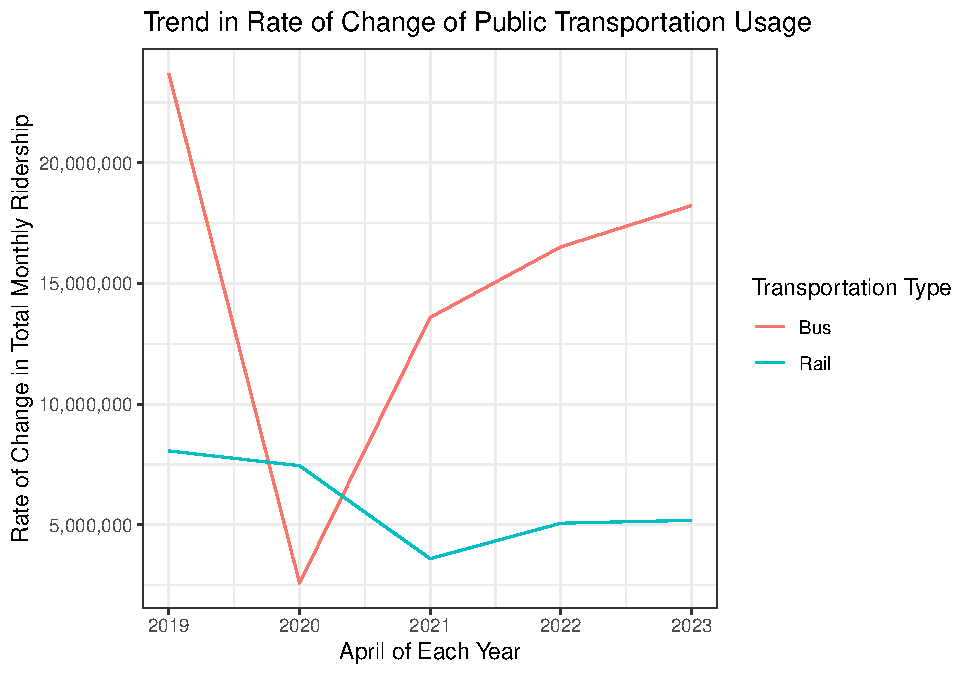
\includegraphics{Paper_files/figure-latex/rate-of-change-plot-1.pdf}
\caption{Line plot of rate of change in public transportation ridership
over time}
\end{figure}

\newpage

\hypertarget{derivative-analysis}{%
\section{Derivative Analysis}\label{derivative-analysis}}

The rate of change in public transportation usage offers valuable
insights into trends and can help forecast future demand. By
differentiating the ridership data with respect to time, we can obtain
the instantaneous rate of change, which is expressed mathematically as:

\[
R'(t) = \frac{dR}{dt}
\]

where \(R(t)\) represents the ridership at time \(t\). This derivative
analysis provides the velocity of ridership change, indicating whether
usage is increasing or decreasing over time.

It is important to keep in mind the usage of information like such. For
Metro, getting their ridership to pre-pandemic numbers would be a huge
accomplishment in the public transit landscape of Los Angeles. Total
ridership in May 2023 was at 77\% of 2019 levels, and in June 2023, it
was at 81\% of its 2019 pre-pandemic level. When using March of 2020 as
our reference point, we can analyze the potentially differing rates of
change in the ridership of Metro Bus and Metro Rail usage over time.
Over the first year from 2020, the total monthly ridership went down
roughly by roughly 22.5 million users.

\hfill\break

The derivative of bus rider usage in Los Angeles from 2019 to 2022 shows
a gradual recovery in ridership, with consistent year-over-year
increases and efforts to restore pre-pandemic levels. The recovery of
bus ridership in Los Angeles reflects the ongoing efforts of Metro to
improve mobility and public transit accessibility in the region. These
changes indicate a positive trend in bus rider usage, with a focus on
restoring and surpassing pre-pandemic ridership levels.

\begin{table}[!htbp] \centering 
  \caption{Linear Regression Results} 
  \label{} 
\begin{tabular}{@{\extracolsep{5pt}}lcc} 
\\[-1.8ex]\hline 
\hline \\[-1.8ex] 
 & \multicolumn{2}{c}{\textit{Dependent variable:}} \\ 
\cline{2-3} 
\\[-1.8ex] & BusRateOfChange & RailRateOfChange \\ 
\\[-1.8ex] & (1) & (2)\\ 
\hline \\[-1.8ex] 
\hline \\[-1.8ex] 
Observations & 4 & 4 \\ 
R$^{2}$ & 0.319 & 0.184 \\ 
Adjusted R$^{2}$ & $-$0.021 & $-$0.223 \\ 
Residual Std. Error (df = 2) & 13,934,596.000 & 2,498,636.000 \\ 
F Statistic (df = 1; 2) & 0.938 & 0.452 \\ 
\hline 
\hline \\[-1.8ex] 
\textit{Note:}  & \multicolumn{2}{r}{$^{*}$p$<$0.1; $^{**}$p$<$0.05; $^{***}$p$<$0.01} \\ 
\end{tabular} 
\end{table}

\begin{table}[!htbp] \centering 
  \caption{Polynomial Regression Results} 
  \label{} 
\begin{tabular}{@{\extracolsep{5pt}}lcc} 
\\[-1.8ex]\hline 
\hline \\[-1.8ex] 
 & \multicolumn{2}{c}{\textit{Dependent variable:}} \\ 
\cline{2-3} 
\\[-1.8ex] & BusRateOfChange & RailRateOfChange \\ 
\\[-1.8ex] & (1) & (2)\\ 
\hline \\[-1.8ex] 
\hline \\[-1.8ex] 
Observations & 4 & 4 \\ 
R$^{2}$ & 0.806 & 0.243 \\ 
Adjusted R$^{2}$ & 0.418 & $-$1.272 \\ 
Residual Std. Error (df = 1) & 10,522,144.000 & 3,405,367.000 \\ 
F Statistic (df = 2; 1) & 2.076 & 0.160 \\ 
\hline 
\hline \\[-1.8ex] 
\textit{Note:}  & \multicolumn{2}{r}{$^{*}$p$<$0.1; $^{**}$p$<$0.05; $^{***}$p$<$0.01} \\ 
\end{tabular} 
\end{table}

\[ \text{Total\ Monthly\ Bus} = -16456298.50 + 6036028.40 \cdot (Year - 2019) \]\[ \text{Total\ Monthly\ Rail} = -2597795.50 + 751531.80 \cdot (Year - 2019) \]\[ \text{Total\ Monthly\ Bus} = -58111913.49 + 33688766315.52 \cdot (Year - 2019) + -8331123.00 \cdot (Year - 2019)^2 \]\[ \text{Total\ Monthly\ Rail} = -239513.00 + -1906155697.79 \cdot (Year - 2019) + 471656.50 \cdot (Year - 2019)^2 \]

\begin{figure}
\centering
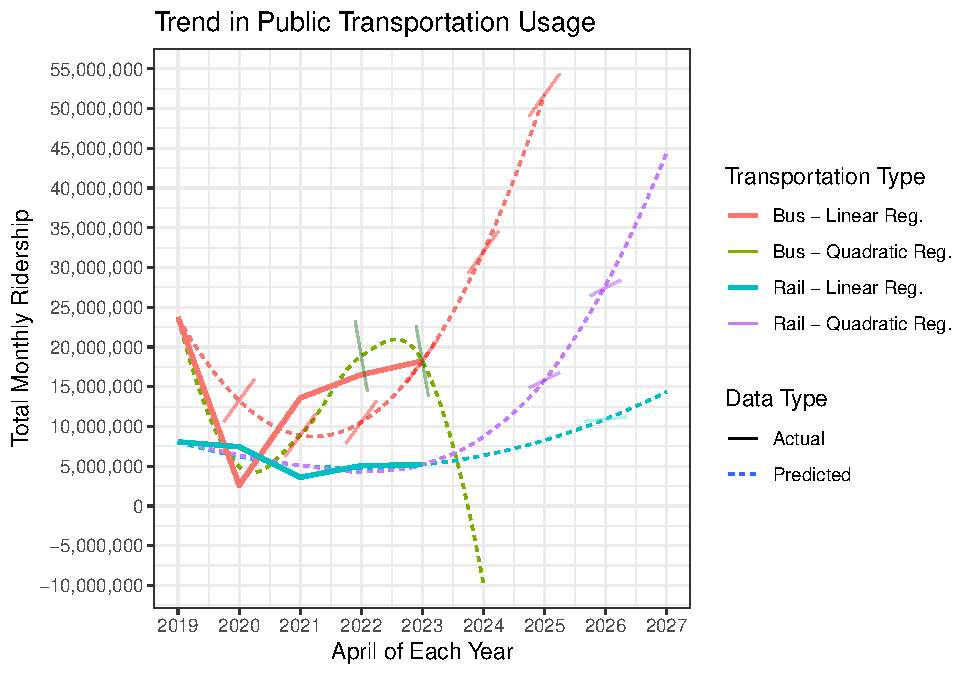
\includegraphics{Paper_files/figure-latex/plot-trend-usage-1.pdf}
\caption{Line plot of public transportation ridership over time with
regression lines}
\end{figure}

\newpage

\hypertarget{conclusion}{%
\subsection{Conclusion}\label{conclusion}}

As previously stated, the aim of this study was to examine how the rapid
growth of Los Angeles affects the demand for public transportation. Our
quantitative research examines the rate of change for transportation
options in Los Angeles based on pricing, availability, convenience, and
modes. With that, as this project was done with the principles of
Business Calculus in mind, it is important to highlight and emphasize
the importance of understanding the applications from our findings.~

\hfill\break

Firstly, an improved understanding of the allocation of resources and
labor is something that decision makers within the public transportation
sector can take away from our analysis. Understanding the rate of change
helps city planners anticipate changes in transportation preferences and
adjust infrastructure investments accordingly. On the projects page of
the metro website (\url{https://www.metro.net/projects/}), there are
dozens of various projects that each require valuable tax-dollars, time,
resources, planning, and execution. As Los Angeles is the third largest
metropolitan area by GDP, being efficient in its decision making
surrounding the allocation of resources in all facets of public
transportation is something that our analysis of the rate of change of
the bus and rail ridership over a five-year period will help better
inform.~

\hfill\break

As anyone who has been to Los Angeles knows the horror stories of its
infamous traffic, our analysis of the rate of change for transportation
options in Los Angeles can guide policies aimed at managing traffic
congestion, an example of such being incentives for alternative
transportation modes. As transportation is a significant contributor to
air pollution and greenhouse gas emissions, understanding how demand for
different transportation options impacts the environment can help in
designing policies that encourage environmentally friendly modes of
transportation, such as public transit or electric vehicles. In a more
economic sense, the transportation sector is closely tied to the overall
economy. Understanding the rate of change can provide insights into the
economic impact of specific changes in transportation options. This
information is valuable for businesses, urban development, and job
accessibility.

\hfill\break
Overall, an analysis of the data of public transportation in a city like
Los Angeles offers immense benefits. From the perspective of the city,
having a clearer understanding of the rate of change between
transportation modes over a five-year period enables them to make better
informed decisions compared to only looking at raw data and trusting
government intuition. From a business and entrepreneurial perspective,
understanding the historical and predicted demand of various
transportation and pricing options allows for entrepreneurs to better
understand the institutional voids that may exist in public
transportation in Los Angeles, and to potentially develop the next
problem solver. (reference proposed Union Station to Dodger Stadium
5,000 seat gondola estimated well over original \$300 million estimate
(\href{https://www.latimes.com/sports/story/2023-04-30/dodger-stadium-gondola-project-frank-mccourt}{latimes.com
-Dodger Stadium Gondola})

\newpage

\hypertarget{sources}{%
\section{Sources:}\label{sources}}

\begin{itemize}
\tightlist
\item
  Transit ridership data: Los Angeles Metro ``L.A. METRO TRANSIT
  RIDERSHIP UP 10 PERCENT, SETS POST-PANDEMIC RECORD'', Patrick Chandler
\item
  Dodger Stadium Gondola Project Proposal
  \href{https://www.latimes.com/sports/story/2023-04-30/dodger-stadium-gondola-project-frank-mccourt}{latimes.com}
\item
  Los Angeles Metro Projects
  \href{https://www.metro.net/projects/}{Metro Projects}
\item
  R Paper source code:
  \url{https://github.com/thatonecalculator/math-28-project}
\end{itemize}

\end{document}
